\documentclass{standalone}
\usepackage{tikz}
\usepackage{rotating}

\usetikzlibrary{shapes, arrows, babel}

\begin{document}
	\begin{turn}{90}
		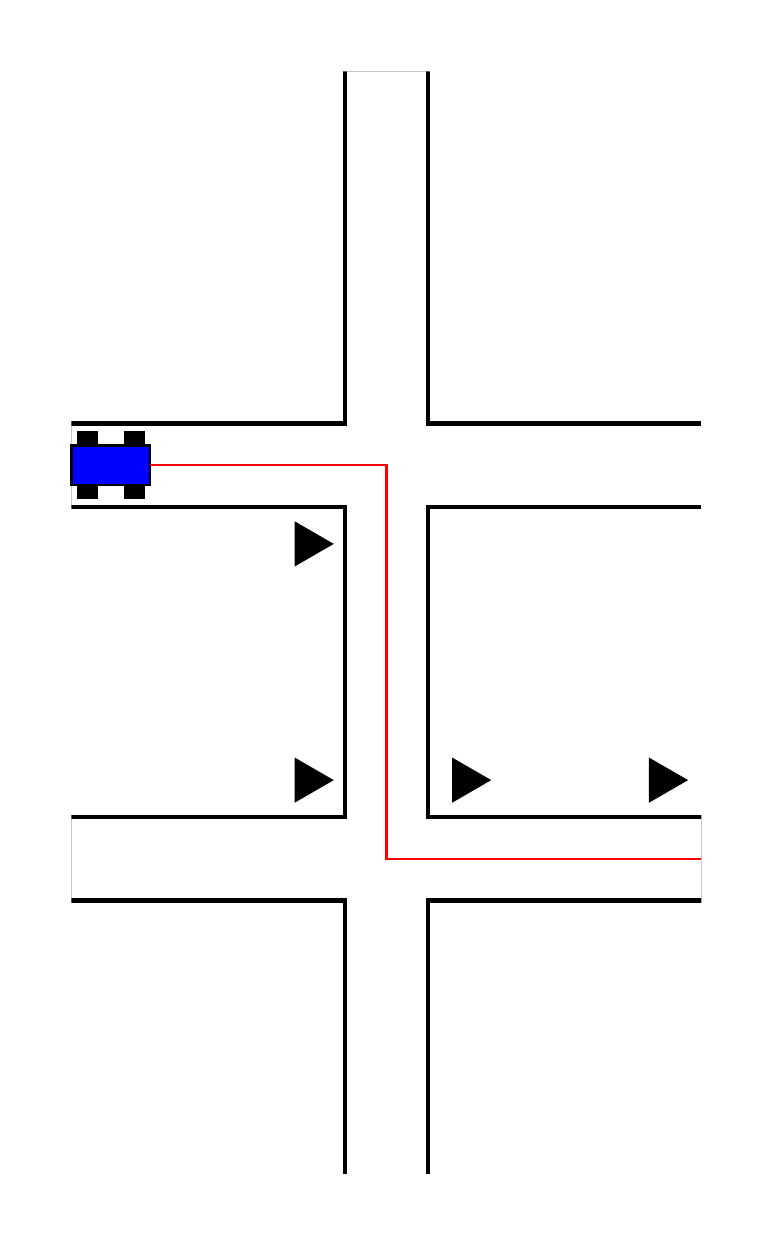
\begin{tikzpicture}
		\draw[double=white,double distance=1cm,ultra thick] (0, 0)--(0, 14)--(0, 4)to[out=180, in=90, looseness=0](-4, 4)--(4, 4)--(0, 4)--(0, 9)to[out=180, in=90, looseness=0](-4, 9)--(4, 9);
		\node(L1) at (-3.2, 9.3)[rectangle, draw, thick, fill=black, minimum width=0.1cm, minimum height=0.1cm]{};
		\node(L2) at (-3.2, 8.7)[rectangle, draw, thick, fill=black, minimum width=0.1cm, minimum height=0.1cm]{};
		\node(L3) at (-3.8, 9.3)[rectangle, draw, thick, fill=black, minimum width=0.1cm, minimum height=0.1cm]{};
		\node(L4) at (-3.8, 8.7)[rectangle, draw, thick, fill=black, minimum width=0.1cm, minimum height=0.1cm]{};
		\node(ROBOT) at (-3.5, 9)[rectangle, draw, thick, fill=blue, minimum width=1cm, minimum height=0.5cm]{};
		\draw[thick,red] (-3, 9)--(0, 9)--(0, 4)--(4, 4);
		\node(S1) at (-1, 8) [regular polygon,regular polygon sides=3,fill=black,minimum height=0.4cm, rotate=30]{};
		\node(S2) at (-1, 5) [regular polygon,regular polygon sides=3,fill=black,minimum height=0.4cm, rotate=30]{};
		\node(S3) at (1, 5) [regular polygon,regular polygon sides=3,fill=black,minimum height=0.4cm, rotate=30]{};
		\node(S4) at (3.5, 5) [regular polygon,regular polygon sides=3,fill=black,minimum height=0.4cm, rotate=30]{};
		\end{tikzpicture}
	\end{turn}
\end{document}